\documentclass[10pt,draftclsnofoot,onecolumn,letterpaper,compsoc]{IEEEtran}

\usepackage[margin=0.75in]{geometry}
\usepackage{float}
\usepackage{graphicx}
\usepackage{caption}
\usepackage{hyperref}
\usepackage{enumerate}
\usepackage{tabu}
\usepackage[english]{babel}\usepackage[numbers]{natbib}
\usepackage{natbib}
\usepackage{longtable}
\usepackage{vhistory}
\usepackage{pgfgantt}
\usepackage{listings}
\usepackage{color}
\usepackage{pdfpages}
\usepackage{lscape}



\lstdefinestyle{mystyle}{
	backgroundcolor=\color{backcolour},   
	commentstyle=\color{codegreen},
	keywordstyle=\color{magenta},
	numberstyle=\tiny\color{codegray},
	stringstyle=\color{codepurple},
	basicstyle=\footnotesize,
	breakatwhitespace=false,         
	breaklines=true,                 
	captionpos=b,                    
	keepspaces=true,                 
	numbers=left,                    
	numbersep=5pt,                  
	showspaces=false,                
	showstringspaces=false,
	showtabs=false,                  
	tabsize=2
}
\lstset{style=mystyle}
\renewcommand{\linespread}{1.0}
\renewcommand{\bibsection}{}

\lstset{
captionpos=b,           
}
\title{Letter of Recommendation Website}
\author{
  \IEEEauthorblockN{Group 8: Letter of Recommendation Website\\Lorenzo Ayala, Scott Waddington, Matthew Kottre, Mingwei Gao, Johnathan Lee} \\
  \IEEEauthorblockA{CS 463: Senior Capstone Spring 2019 \\ Oregon State University}
}
\date{}

\IEEEtitleabstractindextext{
 \begin{abstract}
     The purpose of this document is to provide a review of our project while also providing details to prepare our client, as well as others, to utilize our apps capabilities within one document. Included in the hand off file are all of our documentation throughout all three terms with relation to our project inclusive of weekly blog posts to show team members perspectives and progress. We will wrap up the report with individual reflections by each team member and the valuable skills they learned during the senior capstone experience. 
 \end{abstract}
}

\begin{document}
    %intro page with info and abstract
    \maketitle
    \newpage
    
    %set up table of contents
    \tableofcontents
    \newpage
    
    %brief intro on project
    \section{Brief Introduction}
    Oregon State University has rapidly growing student population, with such an increase professors have been over encumbered by requests for letters of recommendation. In order to remedy the issue, professor Justin Wolford provided the team the solution of developing a web application to allow student's and professors to collaborate in the process of creating letters of recommendation.As a result of this project the teams was able to learn value web development skills that can be translated to future job positions while also being exposed to some industry utilized tools. Throughout the rest of the file you will find all the documentation developed during our time with the project as well as other necessary artifacts to help provide information to our client and end users.\\
    \newpage
    
    %structure and include other doccments for this file
    \section{Problem Statement}
        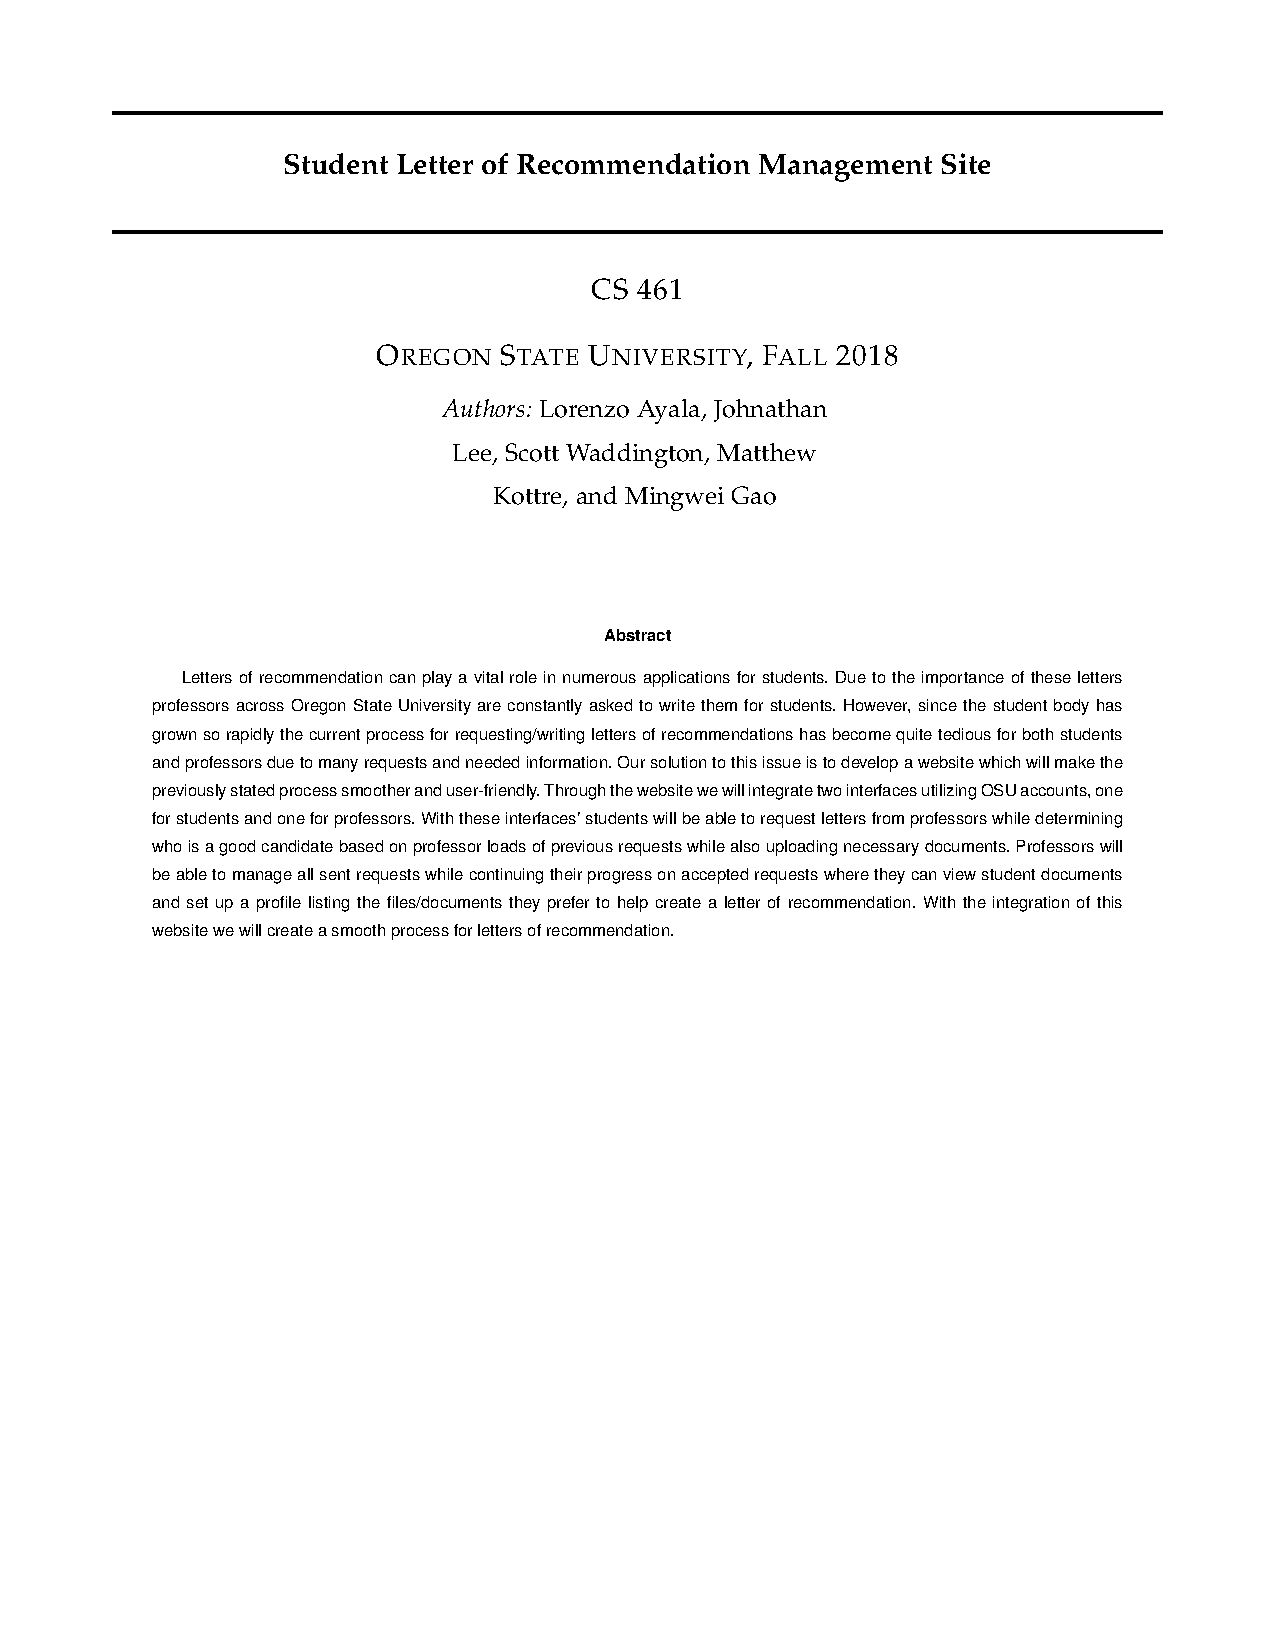
\includepdf[pages=-]{InputDocs/ProblemStatement.pdf}
    \newpage
    
    \section{Requirements Document}
        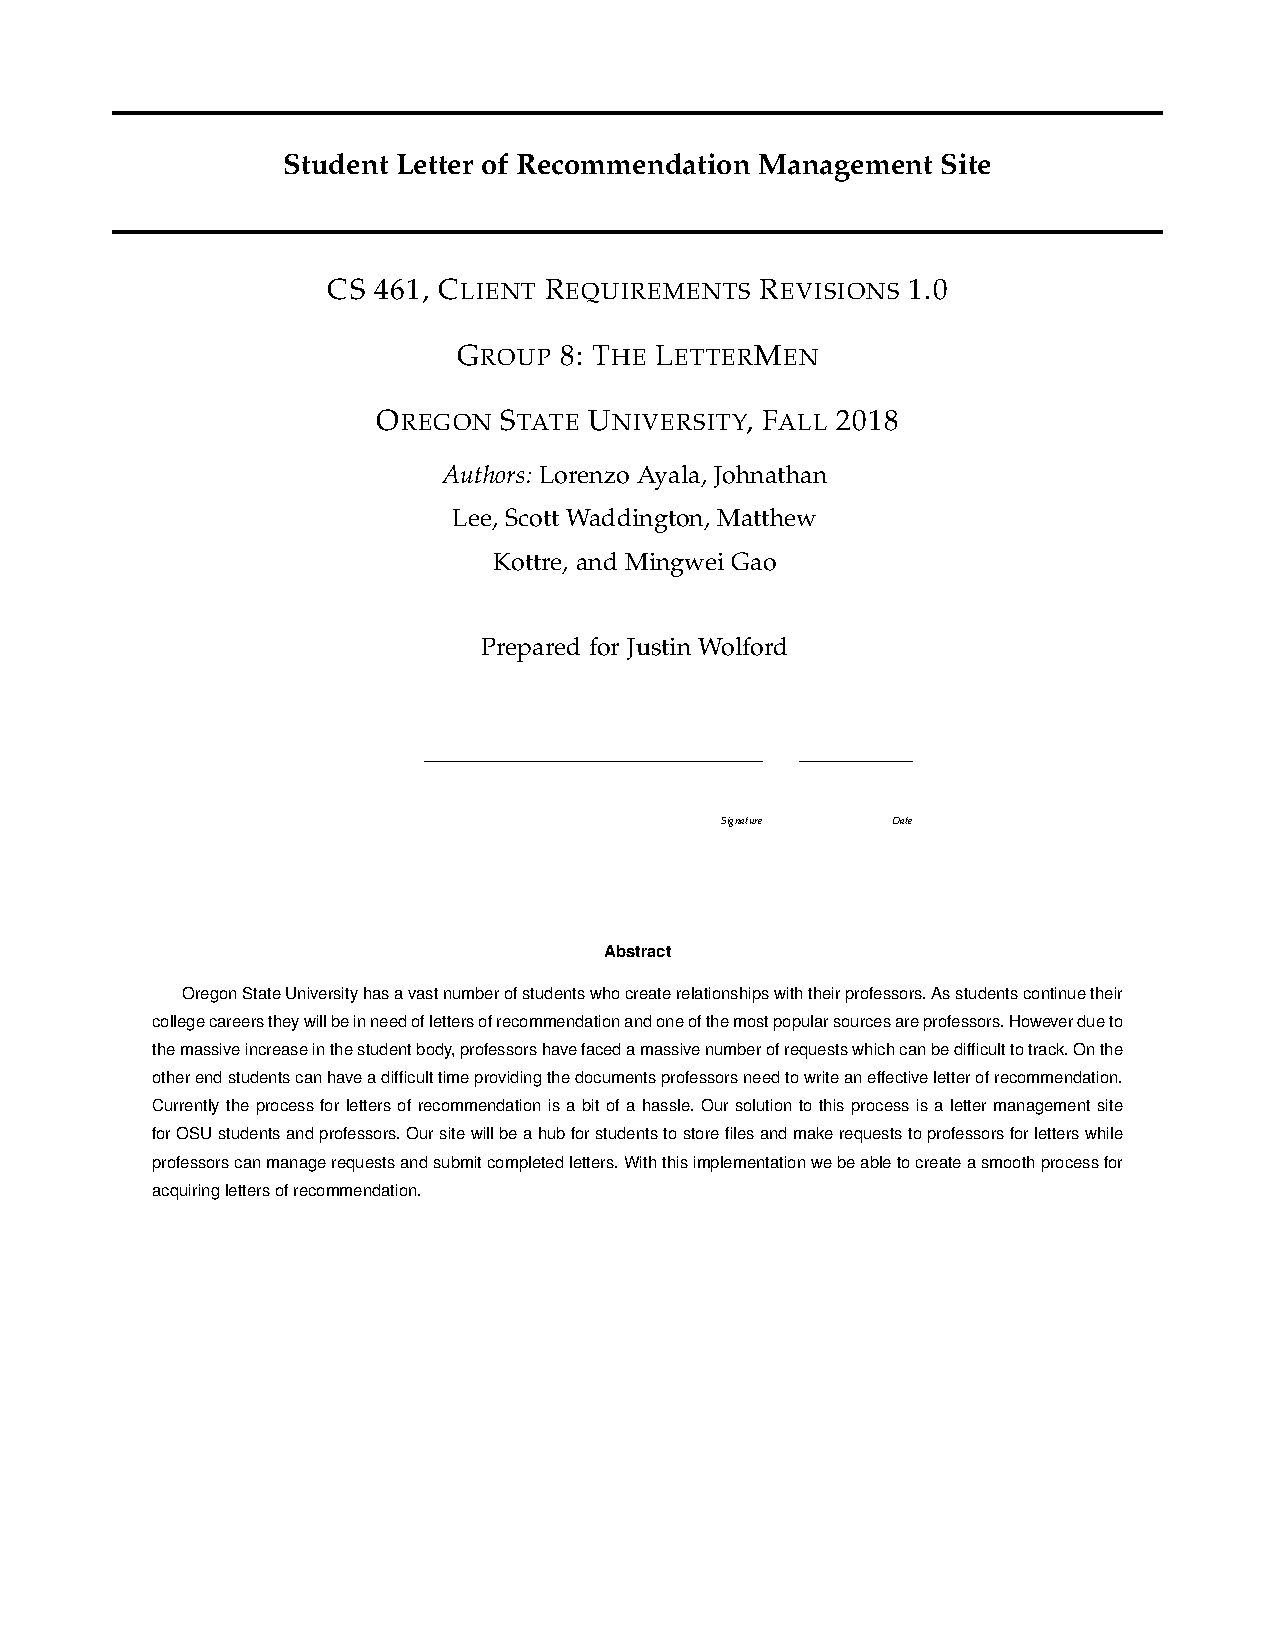
\includepdf[pages=-]{InputDocs/RevisedRequirements.pdf}
    \newpage
    
    \section{Design Document}
        
\includepdf[pages=-]{InputDocs/RevisedDesign.pdf}
    \newpage
    
    \section{Weekly Blogs}
        \subsection{Fall}
\subsubsection{Week 4}

\textbf{Lorenzo Ayala}\\
\noindent\textit{Progress since last week:}\\
For Group 8 who is handling the letter of recommendation site, week 4 went great! I met up with our client to discuss the groups concept of the situation and solution for it which met up with the clients view as well. All members of the group worked with each other efficiently setting up meetings to discuss current/future documents and how we are going to handle responsibilities.\\

\noindent\textit{Any problems you encountered:}\\
\noindent In terms of problems I have none to report as the team members are very easy to get along with and are hard working.\\

\noindent\textit{Plans for the coming week:}\\
\noindent Future plans right now simply consist of continuing our work on future documents such as our requirements document and submitting the final version of our problem statement. Overall not to much to report at this moment but good progress and planning has been made.\\

\noindent\textbf{Johnathan Lee}\\
\noindent\textit{Progress:}\\
A couple of our members met up after class on Tuesday. I did not know they were doing that so unfortunately I was unable to attend. I sent an email requesting to meet up again on Thursday which we did. I got caught up with details about the client, the requirements, and our plans for our final draft of the problem statement. Lorenzo said that he would email us a final version of the problem statement report and told us to look over it whenever we could so we could talk about it during our meetup again with our TA on Friday. The final version looks good and we have done our work for this week. We have a functional github with all of our problem statements in there and we’re planning on using it as version control (just storing all of our stuff for the project in there).\\

\noindent\textit{Problems:}\\
\noindent No problems so far.\\

\noindent\textit{Plans:}\\
\noindent Will probably make contact to meet up again next week so we can draft a requirements document. We still haven’t made a final decision on what kind of language we want to use for this project as the client left it pretty open-ended for us to choose.\\

\noindent\textbf{Matthew Kottre}\\
\noindent\textit{Progress:}\\
We met up as a team a couple of times this week to discuss the project in general as well as the final problem statement. We also met with Wesley, our TA on Friday.\\

\noindent\textit{Problems:}\\
\noindent We have not had any problems yet.\\

\noindent\textit{Plans:}\\
\noindent We only have rough plans for the requirements document so far.\\

\noindent\textbf{Scott Waddington}\\
\noindent\textit{Progress:}\\
This week our group met up 3 times to discuss planning the project as well as writing the problem statement and the requirements document draft. We are meeting with Wesley, our TA, at the library today at 1500. We also heard back from our client, who met with Lorenzo, while the rest of us couldn't make that meeting due to conflict. We plan to meet with him possibly next week.\\

\noindent\textit{Problems:}\\
\noindent None this week.\\

\noindent\textit{Plans:}\\
\noindent We plan to get started on the requirements doc this weekend and finish it next week.\\

\noindent\textbf{Mingwei Gao}\\
\noindent\textit{Progress:}\\
alk with teammates about our group final problem statement on Tuesday and Thursday. By summarizing our five members work we did last week, finally made a new one. Then, we talk with our group TA Wesley this Friday, ask him some question about what should we prepare for the future and he give us some advice about how can we do for the next document.\\

\noindent\textit{Problems:}\\
\noindent Lorenzo asks some questions about what our school service have that we need use for web design and any details that project needs to be considered like matrix design, networking connection.\\

\noindent\textit{Plans:}\\
\noindent we plan to meet each other every week with flexible time. And discuss what should we do for the next assignment.\\

\subsubsection{Week 5}

\textbf{Lorenzo Ayala}\\
\noindent\textit{Progress since last week:}\\
Sorry for the late post completely forgot about this. Progress is going good we are continuing on our documents for the course as required.\\

\noindent\textit{Any problems you encountered:}\\
\noindent No problems at all with the project so everything is going smoothly.\\

\noindent\textit{Plans for the coming week:}\\
\noindent In terms of plans we are just working on future documents which are required for our project and discussing the finer details as a group.\\

\noindent\textbf{Johnathan Lee}\\
\noindent\textit{Progress:}\\
Lorenzo volunteered to take care of the requirements documentation. The due date was pushed back, so there’s no rush. We briefly discussed about the tech review and I went up with Lorenzo to ask the professor some clarifying questions about the tech review and requirements doc.  I was the only one who showed up to meet up with Wesley on Friday.\\

\noindent\textit{Problems:}\\
\noindent No problems so far.\\

\noindent\textit{Plans:}\\
\noindent We can discuss the tech review next week with our entire group. We will look over the requirements documentation and turn that in whenever that’s due.\\

\noindent\textbf{Matthew Kottre}\\
\noindent\textit{Progress:}\\
We have not done much this week other than begin work on the requirements document.\\

\noindent\textit{Problems:}\\
\noindent A potential problem that we may have is for the technology reviews. Since our project is a website, we do not know how to break it into 15 pieces. It is a relatively simple and straightforward concept, so we have only been able to break it into about five pieces so far.\\

\noindent\textit{Plans:}\\
\noindent We will further discuss the tech review to try and break it up further.\\

\noindent\textbf{Scott Waddington}\\
\noindent\textit{Progress:}\\
We have a GitHub repo which includes our individual problem statement papers and tex files, as well as our group statement. We are meeting with our TA today at 1500, but I won't be able to attend this meeting as I have an event I need to be at during that time. We aim to be close to finishing the requirements draft on Monday, and finish the draft after Tuesday's class.\\

\noindent\textit{Problems:}\\
\noindent None.\\

\noindent\textit{Plans:}\\
\noindent As previously mentioned, we plan to have the requirements draft mostly complete by Monday.\\

\noindent\textbf{Mingwei Gao}\\
\noindent\textit{Progress:}\\
 Because I have the midterm on Friday, I would not meet our project, TA Wesley. Also, Ayala has family coming this Friday, the meeting of this week should be canceled. Because of the requirement document deadline extend to next Tuesday. Our team may talk about it online through google hangout this weekend. Then, start work on the next four day.\\

\noindent\textit{Problems:}\\
\noindent Some detail about database design like what we have on our website, still not make sense, I would ask TA in the next meeting time.\\

\noindent\textit{Plans:}\\
\noindent finish requirement document before next Monday and maybe ask TA help us take look at our work. Prepare the Tech review draft1.\\

\subsubsection{Week 6}

\textbf{Lorenzo Ayala}\\
\noindent\textit{Progress since last week:}\\
Currently everything is going well for the team and the project. we are all working on our necessary documents and have completed what was needed for this week. \\

\noindent\textit{Any problems you encountered:}\\
\noindent No issues have arose at all, everyone on the team gets a long pretty well which is great.\\

\noindent\textit{Plans for the coming week:}\\
\noindent Our plans for the following weeks are to continue working on our paper work as needed and meet up to define our project to smaller details.\\

\noindent\textbf{Johnathan Lee}\\
\noindent\textit{Progress:}\\
Lorenzo finished the requirements documentation, we finished the team standards and we finished the tech review. \\

\noindent\textit{Problems:}\\
\noindent No problems so far.\\

\noindent\textit{Plans:}\\
\noindent We can discuss about the project more in depth next week.\\

\noindent\textbf{Matthew Kottre}\\
\noindent\textit{Progress:}\\
This was a relatively slow week for our team. We only met up in class on Tuesday to do the Team Standards activity. We were all on the same page with what to expect and do not foresee any major problems with communication. We briefly discussed the tech review, but since there are five of us, we accepted that there was going to be some overlap in topics. We made sure to do our own work though.\\

\noindent\textit{Problems:}\\
\noindent We did not have any problems this week.\\

\noindent\textit{Plans:}\\
\noindent Next week also looks like it is going to be pretty slow.\\

\noindent\textbf{Scott Waddington}\\
\noindent\textit{Progress:}\\
This week we completed the requirements draft as well as the individual tech reviews and the group expectations table, which we signed off on.\\

\noindent\textit{Problems:}\\
\noindent None.\\

\noindent\textit{Plans:}\\
\noindent I hope to get an early start on next week's work, and start doing some more research on some of the technologies I looked into while writing the tech review.\\

\noindent\textbf{Mingwei Gao}\\
\noindent\textit{Progress:}\\
 Our group makes the requirements document draft1 this week. We discuss the basic process about what we need prepare for future work. Also, think about how to modify our infrastructure if our customer has different requirements. Also, we made the team standards for everyone that make a foundation for planning future work. Because our project TA is busy, we haven't asked him any meeting time, we will make an appointment with him next week.\\

\noindent\textit{Problems:}\\
\noindent Nothing special.\\

\noindent\textit{Plans:}\\
\noindent  I am on the process of prepares the database flow chart since our main work is making the website management. If they have any advise, we can change it in time.\\

\subsubsection{Week 7}

\textbf{Lorenzo Ayala}\\
\noindent\textit{Progress since last week:}\\
Sorry for yet another late submission I completely forgot about this again. Overall everything is going well the team has completed all recent assignments.\\

\noindent\textit{Any problems you encountered:}\\
\noindent There are no issues whatsoever the team works well together I still do not see any problems in the future.\\

\noindent\textit{Plans for the coming week:}\\
\noindent In terms of plans the team will soon begin working on the Design Document which will be released for week 8 and I believe things will go smoothly with the document as well.\\

\noindent\textbf{Johnathan Lee}\\
\noindent\textit{Progress:}\\
Finished the tech review. Individual assignments meant we did not need to communicate with each other this week.\\

\noindent\textit{Problems:}\\
\noindent No problems so far.\\

\noindent\textit{Plans:}\\
\noindent No current plans. Can research about coding methods for the project on our own.\\

\noindent\textbf{Matthew Kottre}\\
\noindent\textit{Progress:}\\
This was a slow week for us and we did not meet up at all. I only worked on the final draft of my Tech Review.\\

\noindent\textit{Problems:}\\
\noindent We did not have any problems this week.\\

\noindent\textit{Plans:}\\
\noindent We will most likely meet next week to discuss the design document.\\

\noindent\textbf{Scott Waddington}\\
\noindent\textit{Progress:}\\
This week we worked individually on our tech reviews. We didn't get to meet with our TA today because he was busy today and unable to meet with any of his groups.\\

\noindent\textit{Problems:}\\
\noindent None.\\

\noindent\textit{Plans:}\\
\noindent We plan to start looking into the design document once its module is available to be viewed.\\

\noindent\textbf{Mingwei Gao}\\
\noindent\textit{Progress:}\\
The main work this week is the individual Tech Review, and because our project just has a few technical elements need to consider. So, after we share the point with each teammate, we may write the same thing with different description when we doing the Tech Review. Also, the team leader doesn't tell us the next step, so, we may meet each other next week.\\

\noindent\textit{Problems:}\\
\noindent The specific problem needs to be considered in Tech Review already solved in our class. Everything should be fine.\\

\noindent\textit{Plans:}\\
\noindent meet team and project TA next week and take look at the Design Document this weekend.\\

\subsubsection{Week 8}

\textbf{Lorenzo Ayala}\\
\noindent\textit{Progress since last week:}\\
For week 8 things still continue to go smoothly. With the release of the design document the group has had a brief of discussion on the documents organization and we will continue discussion on the progress of the document and writing responsibilities as well as the content to be included.\\

\noindent\textit{Any problems you encountered:}\\
\noindent Problems have not occurred at all and still do not see any to occur as the team gets a long very well together.\\

\noindent\textit{Plans for the coming week:}\\
\noindent Plans will continue to rotate around the design document as we progress to develop the document around our project and we will begin to develop the progress report document and media after completion of the design document.\\

\noindent\textbf{Johnathan Lee}\\
\noindent\textit{Progress:}\\
Nothing to report.\\

\noindent\textit{Problems:}\\
\noindent No problems so far.\\

\noindent\textit{Plans:}\\
\noindent We may plan on meeting to talk more about the project and see what other group members have done. An email may suffice as well.\\

\noindent\textbf{Matthew Kottre}\\
\noindent\textit{Progress:}\\
This was another slow week for us. We briefly discussed what we have been doing and some initial plans for the design document after class on Thursday. Other than that, we didn't do anything else this week.\\

\noindent\textit{Problems:}\\
\noindent We did not have any problems this week.\\

\noindent\textit{Plans:}\\
\noindent We will most likely meet next week to discuss our current progress.\\

\noindent\textbf{Scott Waddington}\\
\noindent\textit{Progress:}\\
We didn't do much as a group this week, as there wasn't anything due.\\

\noindent\textit{Problems:}\\
\noindent None.\\

\noindent\textit{Plans:}\\
\noindent We plan to look at the design document individually over this next week. We likely won't have a team meeting due to the week being so short. We will remain in communication electronically.\\

\noindent\textbf{Mingwei Gao}\\
\noindent\textit{Progress:}\\
 still on the process checking my Tech review have been graded, also spend some time reading technical support article about PHP and database design of web build to prepare my design document. And Ta asks us about the meeting time talking about the "problem statement" content supplement next week.\\

\noindent\textit{Problems:}\\
\noindent  I still have no idea should we include what kind of web security level in our project. And I am not very familiar with web security. So, I may list some question about that.\\

\noindent\textit{Plans:}\\
\noindent  Revised the article until it met with professor's satisfaction and read more article about web security.\\

\subsubsection{Week 9}

\textbf{Lorenzo Ayala}\\
\noindent\textit{Progress since last week:}\\
As of week 9 progress continues on the design document as all members work on their own segment of the document and discussion continues on the progress report which should be straight forward.\\

\noindent\textit{Any problems you encountered:}\\
\noindent No problems have occurred yet and everything should still go smoothly as expected.\\

\noindent\textit{Plans for the coming week:}\\
\noindent Future plans consist of working on our design document and the progress report so that we can complete this terms assignments.\\

\noindent\textbf{Johnathan Lee}\\
\noindent\textit{Progress:}\\
Week of Thanksgiving, progress is slowed. Haven’t exactly done anything this week.\\

\noindent\textit{Problems:}\\
\noindent No problems so far.\\

\noindent\textit{Plans:}\\
\noindent We are making plans to help with the creation of the video that showcases our progress so far. Our design document is being worked on, we have decided that it won't be very hard to do as it seems to be mostly a compilation of the work we have done already.\\

\noindent\textbf{Matthew Kottre}\\
\noindent\textit{Progress:}\\
I have not been on campus this week because I am home for Thanksgiving. We were not able to meet up because of this. I started working on the design document from the brief discussions we had after class on Thursday. I have not gotten very far on it yet and am planning on doing most of it this weekend.\\

\noindent\textit{Problems:}\\
\noindent We did not have any problems this week.\\

\noindent\textit{Plans:}\\
\noindent We will discuss plans for the progress report video.\\

\noindent\textbf{Scott Waddington}\\
\noindent\textit{Progress:}\\
We didn't meet this week since we had a really short week. We are looking over and starting the design document draft this weekend and we will meet as a group before it's due next week.\\

\noindent\textit{Problems:}\\
\noindent None.\\

\noindent\textit{Plans:}\\
\noindent We plan to meet early next week to finish up the design draft and look at the remaining assignments for the term.\\

\noindent\textbf{Mingwei Gao}\\
\noindent\textit{Progress:}\\
 The writing center only can make the one-hour appointment every time. That's not enough for my technical review modification. The writing center worker checked half of my file they ask me to come again next week. Also, I email my teammates ask their thought about the design document, still waiting for their response.\\

\noindent\textit{Problems:}\\
\noindent The design document hasn't started yet and still waiting for my teammate's feedback. I made the online word file shared with them. Moreover, create a basic framework for the team.\\

\noindent\textit{Plans:}\\
\noindent finish the technical review modification and submit our design document in time.\\
        \subsection{Winter}
\subsubsection{Week 1}

\textbf{Lorenzo Ayala}\\
\noindent\textit{Progress since last week:}\\
The group has begun discussing meeting times to establish for both group and TA development/discussion.\\

\noindent\textit{Any problems you encountered:}\\
\noindent  No problems at all the group works well together as usual.\\

\noindent\textit{Plans for the coming week:}\\
\noindent After establishing meeting times development on the project will proceed.\\

\noindent\textbf{Johnathan Lee}\\
\noindent\textit{Progress:}\\
Emailing group members to determine a meetup time every week with the TA. \\ 

\noindent\textit{Problems:}\\
\noindent There are time conflicts with the times the TA has given us.\\

\noindent\textit{Plans:}\\
\noindent We can try asking the TA for more times. Otherwise, we may have to schedule a time where not every one of our group members can make it.\\

\noindent\textbf{Matthew Kottre}\\
\noindent\textit{Progress:}\\
There isn't much to report because it is the first week of the term, so we are still working on getting organized.\\

\noindent\textit{Problems:}\\
\noindent A minor problem we are facing is we all have very different schedules this term, which results in us experiencing some difficulty finding a time that we can have our weekly meeting with our TA.\\

\noindent\textit{Plans:}\\
\noindent We will focus on getting organized after the break and find a time that works for all of us to meet up.\\

\noindent\textbf{Scott Waddington}\\
\noindent\textit{Progress:}\\
Our group did not spend any time working on our project over the break. This week we are figuring out a time to meet with out new TA, and comparing schedules to see who is available at what times.\\

\noindent\textit{Problems:}\\
\noindent None.\\

\noindent\textit{Plans:}\\
\noindent We plan to start implementation on the project soon, according to the plans we created last term.\\

\noindent\textbf{Mingwei Gao}\\
\noindent\textit{Progress:}\\
Schedule the meeting time with our Capstone TA Omeed in next week. Start working on my part for project building. Get ready for some questions about database build when we meet the TA.\\

\noindent\textit{Problems:}\\
\noindent Team still not make the final decision for the meeting time next week. And also, the project detail may need to talk with our customer more and get some advice from him.\\

\noindent\textit{Plans:}\\
\noindent  Email my teammates ask their free time next week to meet our TA and ask them whether to make an appointment with our customer.\\


\subsubsection{Week 2}

\textbf{Lorenzo Ayala}\\
\noindent\textit{Progress since last week:}\\
We met up with the TA and discussed the project. Established that 4pm on Wednesdays is our meetup time.\\

\noindent\textit{Any problems you encountered:}\\
\noindent No problems at all with the group or on the project yet.\\

\noindent\textit{Plans for the coming week:}\\
\noindent The group plans to begin development on the project during the three day weekend and continue our weekly Wednesday meetings.\\

\noindent\textbf{Johnathan Lee}\\
\noindent\textit{Progress:}\\
We met up with the TA and discussed the project. Established that 4pm on Wednesdays is our meetup time. \\ 

\noindent\textit{Problems:}\\
\noindent No problems so far.\\

\noindent\textit{Plans:}\\
\noindent Lorenzo mentioned he might start some implementation this weekend and email us.\\

\noindent\textbf{Matthew Kottre}\\
\noindent\textit{Progress:}\\
We have made progress on the early draft of our poster. Having a template made it much easier.\\

\noindent\textit{Problems:}\\
\noindent We haven't had any problems this week other than still working on getting organized for the term.\\

\noindent\textit{Plans:}\\
\noindent Our plans for the week are to work on our elevator pitch and decide what language we want to use for our project. At the meeting with our TA, we discussed possible using either PHP or Python.\\

\noindent\textbf{Scott Waddington}\\
\noindent\textit{Progress:}\\
We met with our TA and are working to get started on implementation. We also discussed elevator pitches and the poster.\\

\noindent\textit{Problems:}\\
\noindent None.\\

\noindent\textit{Plans:}\\
\noindent We plan to start implementation on the project soon, according to the plans we created last term. This weekend we will be working on posters as well.\\

\noindent\textbf{Mingwei Gao}\\
\noindent\textit{Progress:}\\
his week Wednesday is our first time meeting with our project TA. Our group asks him to provide some advice about the project detail and double check every part of our plan is in the right way. And because I am taking CS440 database class, it's good for me to design our database with professor's help.\\

\noindent\textit{Problems:}\\
\noindent None.\\

\noindent\textit{Plans:}\\
\noindent Confirm the teamwork scheduling process next week. Ask my database professor how to design the database to avoid too many user logging crashes the website.\\

\subsubsection{Week 3}

\textbf{Lorenzo Ayala}\\
\noindent\textit{Progress since last week:}\\
For week 3 we have looked at templates we could replicate to create the final product for our project and met up with Omeed to discuss this. \\

\noindent\textit{Any problems you encountered:}\\
\noindent None whatsoever and don't see any in the future.\\

\noindent\textit{Plans for the coming week:}\\
\noindent We will begin implementing our project this weekend and hopefully get a good start on it. \\

\noindent\textbf{Johnathan Lee}\\
\noindent\textit{Progress:}\\
Confirmed that we have class on Tuesday at around 8:40am. Lorenzo created and shared the poster to group members. \\ 

\noindent\textit{Problems:}\\
\noindent No problems so far.\\

\noindent\textit{Plans:}\\
\noindent Make a decent elevator pitch for class.\\

\noindent\textbf{Matthew Kottre}\\
\noindent\textit{Progress:}\\
This was a slow week for us, so we didn't have much progress. We created the poster draft and are currently working on the elevator pitch.\\

\noindent\textit{Problems:}\\
\noindent We haven't had any problems this week.\\

\noindent\textit{Plans:}\\
\noindent This weekend we are planning to finish the elevator pitch. We haven't definitively decided what programming language we are going to use for the implementation yet, but we are leaning towards Python and the Django framework. I am planning on doing some research and a little experience with Django this weekend.\\

\noindent\textbf{Scott Waddington}\\
\noindent\textit{Progress:}\\
Beginning implementation on project. Looking at how to make it work with OSU's authentication system. Completed the poster rough draft\\

\noindent\textit{Problems:}\\
\noindent None.\\

\noindent\textit{Plans:}\\
\noindent Continue to work on the project. Will be ready for the elevator pitch next week.\\

\noindent\textbf{Mingwei Gao}\\
\noindent\textit{Progress:}\\
 This week team complete the early poster of our project. For our project, I can complete the fundamental database structure this weekend. \\

\noindent\textit{Problems:}\\
\noindent None.\\

\noindent\textit{Plans:}\\
\noindent  Next week Tuesday, prepare team elevator patch and finish the basic structure of project database design. Then, ask some advice from team member after they take a look. Asking other teammates overseeing their part and review their recent process.\\

\subsubsection{Week 4}

\textbf{Lorenzo Ayala}\\
\noindent\textit{Progress since last week:}\\
For this week we have began developing the application for our client with further development happening.\\

\noindent\textit{Any problems you encountered:}\\
\noindent Not at all as usual.\\

\noindent\textit{Plans for the coming week:}\\
\noindent The group plans on meeting this weekend to delegate responsibilities for each other and continue working on our project. \\

\noindent\textbf{Johnathan Lee}\\
\noindent\textit{Progress:}\\
We're using Django for our project. We found a group to do our poster critique. \\ 

\noindent\textit{Problems:}\\
\noindent No problems so far.\\

\noindent\textit{Plans:}\\
\noindent We are currently in the middle of an email thread to confirm a time that everyone is good with in both groups. I believe we have a time or are very close to securing a time.\\

\noindent\textbf{Matthew Kottre}\\
\noindent\textit{Progress:}\\
I followed the tutorial on the Django website to familiarize myself with the framework. We found another group to do the poster critique with and are working on organizing a time that works for everyone.\\

\noindent\textit{Problems:}\\
\noindent We haven't had any problems this week.\\

\noindent\textit{Plans:}\\
\noindent We are planning on meeting up this weekend to discuss our plans and begin our implementation.\\

\noindent\textbf{Scott Waddington}\\
\noindent\textit{Progress:}\\
We have a basic layout of the front-end and are continuing to work on the back-end of the website and develop the database.\\

\noindent\textit{Problems:}\\
\noindent I attended the required class period to go over elevator pitches and turned in the small slip with my noted from that class period, but the elevator pitch assignment is showing as a 0 for me. Dr. Winters said she was going to check her files, but it has been a few days and the grade hasn't been changed.\\

\noindent\textit{Plans:}\\
\noindent We are going to keep working on the project and we are planning to meet as a group this weekend to see where we are at.\\

\noindent\textbf{Mingwei Gao}\\
\noindent\textit{Progress:}\\
This week team participates the elevator pitch and share the project information with other teams. During the pitch time, our team also find another group would come prepares the poster critique activity with us next week. For our project, I start reading some advanced database design this week. Also, our team leader Ayala sounds like finish the backend part when we meet during the TA meeting time. Other team members still working on other parts of the project.\\

\noindent\textit{Problems:}\\
\noindent Everything is good. Kirsten said, we need work 12 hours per week, I think I need to work harder. Again, the only problem I am worried about is the project schedule. \\

\noindent\textit{Plans:}\\
\noindent Both group still discuss the appropriate time of poster critique activity next week. We will make the final decision Friday before the due time. My plan for next week is to figure out how is my database design and whether need modify and perfect.\\

\subsubsection{Week 5}

\textbf{Lorenzo Ayala}\\
\noindent\textit{Progress since last week:}\\
We have started developing features of our app  which were delegated among team members.\\

\noindent\textit{Any problems you encountered:}\\
\noindent None at all and none can be seen in the future.\\

\noindent\textit{Plans for the coming week:}\\
\noindent The group plans on meeting with our client to setup the CAS login so we can continue development.\\

\noindent\textbf{Johnathan Lee}\\
\noindent\textit{Progress:}\\
We did our poster critique with another group. I got my Django set up and am currently working on the website. \\ 

\noindent\textit{Problems:}\\
\noindent No problems so far.\\

\noindent\textit{Plans:}\\
\noindent Just get some work on the website.\\

\noindent\textbf{Matthew Kottre}\\
\noindent\textit{Progress:}\\
We are now in the very early stages of implementing our project. We have a single page with a basic theme that is mostly just getting Django set up properly.\\

\noindent\textit{Problems:}\\
\noindent Other than the little annoyances of learning a new programming language and framework, there have not been any notable problems.\\

\noindent\textit{Plans:}\\
\noindent We each have a rough idea of what we need to work on in the coming days and weeks. I am currently working on creating a rough template for the scheduling page that instructors will use to keep track of when each letter is due.\\

\noindent\textbf{Scott Waddington}\\
\noindent\textit{Progress:}\\
We have added to the basic server. Personally, I set up a very simple file upload system, which will probably be modified once the database is added.\\

\noindent\textit{Problems:}\\
\noindent None.\\

\noindent\textit{Plans:}\\
\noindent We will continue to work on the server, and will probably see our client sometime in the next 1 or 2 weeks in order to work out the OSU CAS system to get accounts set up on our site.\\

\noindent\textbf{Mingwei Gao}\\
\noindent\textit{Progress:}\\
This week team participates the Poster critique meeting with Professor Kirsten and another team in KEC. Both groups share the feedback about each poster design and professor help us perfect the Poster structure. For our project, I already finish the database design and team ask me to do the backend setup. Since I haven't learn python before, I need to learn it at least one week to start working on it later. Also, other team members sound like working on other parts of the project as well.\\

\noindent\textit{Problems:}\\
\noindent Everything is good. And this week I might need more time work on my midterm review. Project backend setup study will delay after exam finish. After midterm, i would ask my teammates about the plan of making the winter term reporting work.\\

\noindent\textit{Plans:}\\
\noindent Asking my teammates about the design of building the winter term reporting work. Figure out how to set up the backend by python and connect the other part my teammates did in the future.\\

\subsubsection{Week 6}

\textbf{Lorenzo Ayala}\\
\noindent\textit{Progress since last week:}\\
Currently we have our web app functioning with some basic features and have met up with our client Justin to discuss the CAS login setup.\\

\noindent\textit{Any problems you encountered:}\\
\noindent None so far but maybe some in the future with CAS but we have a number of resources to help.\\

\noindent\textit{Plans for the coming week:}\\
\noindent Polish up our web application and look over django CAS packages for implementing the login this next week. \\

\noindent\textbf{Johnathan Lee}\\
\noindent\textit{Progress:}\\
Still just working on the project. \\ 

\noindent\textit{Problems:}\\
\noindent No problems so far.\\

\noindent\textit{Plans:}\\
\noindent Meeting up with our client on Friday to check some miscellaneous things such as CAS setup.\\

\noindent\textbf{Matthew Kottre}\\
\noindent\textit{Progress:}\\
We met with our client this week to discuss our plans integrating with CAS as well as some questions about the URL and hosting. He pointed us towards a project that will likely help us add CAS support. He also gave us the names of some other people we can contact for more information.\\

\noindent\textit{Problems:}\\
\noindent We haven't had any problems this week.\\

\noindent\textit{Plans:}\\
\noindent Our plans for the coming week are to set up our database and get our project to the alpha stage. Our progress may be slightly behind where we should be, but we know what we need to do. There are not any concerns about the timeline.\\

\noindent\textbf{Scott Waddington}\\
\noindent\textit{Progress:}\\
We are continuing to work on developing the website. Personally, I'm waiting on the database portion to be finished so that I can adapt the file upload system.\\

\noindent\textit{Problems:}\\
\noindent I'd like to see the website coming together a little quicker, but overall I'm not that worried about it.\\

\noindent\textit{Plans:}\\
\noindent Continue developing the site, finish the midterm report.\\

\noindent\textbf{Mingwei Gao}\\
\noindent\textit{Progress:}\\
This week i am pretty busy about my midterm and team still working on winter term reporting until we receive the message that Kirsten pushes the due date to next week. For our project, I am starting to build the backend setup this Saturday. I will learn how to do it online while writing the backend setup. I will take a look at our report this weekend, start early for more time working on back-end build part.\\

\noindent\textit{Problems:}\\
\noindent  Everything is good. Midterm finished this week. Project backend setup will keep going. The problems I am worried about is backend setup coding process, right now has too many bugs not fixed, I will try to finish it this weekend.\\

\noindent\textit{Plans:}\\
\noindent Figure out how to fix the backend coding bug and think about how to write winter term report.\\

\subsubsection{Week 7}

\textbf{Lorenzo Ayala}\\
\noindent\textit{Progress since last week:}\\
Still working on the website and also working with Justin on setting up accounts for the CAS login system. \\

\noindent\textit{Any problems you encountered:}\\
\noindent  None really just need to get the team rolling on this project to hammer it out and to get the CAS login setup.\\

\noindent\textit{Plans for the coming week:}\\
\noindent Continue developing the app and work with Justin to finish up gathering the necessary information for the CAS login. \\

\noindent\textbf{Johnathan Lee}\\
\noindent\textit{Progress:}\\
Added a new page, button, and text field. \\ 

\noindent\textit{Problems:}\\
\noindent No problems so far.\\

\noindent\textit{Plans:}\\
\noindent Add more functionality, add more to the website, check up with group members on their progress, make a progress report.\\

\noindent\textbf{Matthew Kottre}\\
\noindent\textit{Progress:}\\
I had a midterm and a project for another class this week, so I didn't get much done on the project this week.\\

\noindent\textit{Problems:}\\
\noindent We haven't had any problems this week.\\

\noindent\textit{Plans:}\\
\noindent There are not any specific plans for the coming week. Just continuing the development. I'll probably try to get Django templates set up so that every page has a consistent design.\\

\noindent\textbf{Scott Waddington}\\
\noindent\textit{Progress:}\\
This week we continued work on the server. We have also contact the CAS team to get our website set up to use OSU's CAS login.\\

\noindent\textit{Problems:}\\
\noindent None.\\

\noindent\textit{Plans:}\\
\noindent We plan to have the database done during the next week so that we can finish implementation. We would also like to have CAS setup by next week.\\

\noindent\textbf{Mingwei Gao}\\
\noindent\textit{Progress:}\\
I forget our meeting time is Wednesday this week since several assignments due this week. For our project, Team still waiting for the answer from our clients. We ask him about the AWS service building since our application interface still need it to complete. I am not busy this weekend and I will focus on our report, and keep working on back-end build part.\\

\noindent\textit{Problems:}\\
\noindent  Everything is good. Project backend setup will keep going. Still waiting for the client response. And finish this winter report this weekend.\\

\noindent\textit{Plans:}\\
\noindent Figure out how to fix the database coding bug and quickly finish it before next week.\\

\subsubsection{Week 8}

\textbf{Lorenzo Ayala}\\
\noindent\textit{Progress since last week:}\\
Currently we are still developing on the redesign while working on setting up personal AWS EC2 instances to prepare our app for deployment.\\

\noindent\textit{Any problems you encountered:}\\
\noindent None really just waiting for the necessary information to setup an EC2 instance through the university so that we can get a url to establish a CAS login. \\

\noindent\textit{Plans for the coming week:}\\
\noindent Continue to develop the functionality of our site so that we can have a smooth migration over to AWS.\\

\noindent\textbf{Johnathan Lee}\\
\noindent\textit{Progress:}\\
Extracted values from text fields. \\ 

\noindent\textit{Problems:}\\
\noindent Don't know how to interact with our database.\\

\noindent\textit{Plans:}\\
\noindent Research into SQL databases, read more into Django documentation, look into other works.\\

\noindent\textbf{Matthew Kottre}\\
\noindent\textit{Progress:}\\
This was a very busy week for me, so I did not get much of a chance to work on the project.\\

\noindent\textit{Problems:}\\
\noindent I am having a few minor problems connecting to the database from Django, but it shouldn't be too difficult to figure it out.\\

\noindent\textit{Plans:}\\
\noindent I plan on trying to connect to the default sqlite database to get the schedule working since our database is not yet finished.\\

\noindent\textbf{Scott Waddington}\\
\noindent\textit{Progress:}\\
This week we have continued our interaction with the OSU CAS team so that we can integrate their login system with our application.\\

\noindent\textit{Problems:}\\
\noindent None.\\

\noindent\textit{Plans:}\\
\noindent Once we get CAS implemented, we can get our database setup to store account data.\\

\noindent\textbf{Mingwei Gao}\\
\noindent\textit{Progress:}\\
 I complete my Database design part this week, I will focus on the PHP setting this weekend. The entire work can be finish before next Tuesday. The team already got the answer from our clients. The Client recommends us to run the whole stack on EC2 or run the database on RDS. The team will get the free year to develop on AWS in the future. \\

\noindent\textit{Problems:}\\
\noindent  According to the feedback of our winter term report, we need adding more screenshot on the interface part and reword some introduction in the project purpose part.\\

\noindent\textit{Plans:}\\
\noindent Figure out the video record work in next week. Correct the problem from the feedback classmate noticed. Review the other problems probably existed.\\

\subsubsection{Week 9}

\textbf{Lorenzo Ayala}\\
\noindent\textit{Progress since last week:}\\
Just refining the pieces that we have for our project while we wait for information regarding the account.\\

\noindent\textit{Any problems you encountered:}\\
\noindent None yet just hoping to hear back from Justin.\\

\noindent\textit{Plans for the coming week:}\\
\noindent Keep refining our pieces and prepare to demo our project for the progress report.\\

\noindent\textbf{Johnathan Lee}\\
\noindent\textit{Progress:}\\
Read up on Django documentation, still looking into redesigning the preferences page. \\ 

\noindent\textit{Problems:}\\
\noindent None.\\

\noindent\textit{Plans:}\\
\noindent Test database functionality with the page.\\

\noindent\textbf{Matthew Kottre}\\
\noindent\textit{Progress:}\\
I connected the schedule to the development sqlite database. It doesn't support multiple users yet, but it should be relatively simple to add that functionality after we get the final database set up.\\

\noindent\textit{Problems:}\\
\noindent The only problem we are having is getting the billing information for AWS. We are doing are development locally, so it isn't that big of a deal presently.\\

\noindent\textit{Plans:}\\
\noindent We are going to work on the database and further refine some of the pages. I want to make some adjustments to the model for the schedule to make it easier to switch to the final database when it is ready.\\

\noindent\textbf{Scott Waddington}\\
\noindent\textit{Progress:}\\
This week we are mostly waiting to hear back from our client so that we can get a billing number for our domain address to our website.\\

\noindent\textit{Problems:}\\
\noindent None.\\

\noindent\textit{Plans:}\\
\noindent Once we get the domain address we can finish the CAS setup and get our application running with a CAS login.\\

\noindent\textbf{Mingwei Gao}\\
\noindent\textit{Progress:}\\
 we plan to modify our winter report according to the feedback from other classmates. They advise us to add more information about what we left. And they want more screenshot with the specific description on it. The team should start working on the improvement process and record video part in next week.\\

\noindent\textit{Problems:}\\
\noindent Right now, we looking good on the way of finishing the basic structure of our project. \\

\noindent\textit{Plans:}\\
\noindent  Team getting Start working on the video record work. Also Reviewing the problem from the feedback and build final report template for the team.\\

\subsubsection{Week 10}

\textbf{Lorenzo Ayala}\\
\noindent\textit{Progress since last week:}\\
We were able to get an account to finance a AWS instance which will soon be set up for prototyping.\\

\noindent\textit{Any problems you encountered:}\\
\noindent None now but setting up CAS could be a future issue during setup.\\

\noindent\textit{Plans for the coming week:}\\
\noindent The team is planning on completing the required progress report and video while also continuing development on our project.\\

\noindent\textbf{Johnathan Lee}\\
\noindent\textit{Progress:}\\
Preferences are being saved. Working on displaying them out. \\ 

\noindent\textit{Problems:}\\
\noindent Running out of time. Should probably spend more time.\\

\noindent\textit{Plans:}\\
\noindent Implement view of preferences. Might want different types of pages for these. The group is planning on meeting up and getting the project together over the weekend.\\

\noindent\textbf{Matthew Kottre}\\
\noindent\textit{Progress:}\\
I've been busy with projects for other classes, so I haven't done much during the last week. I started on an info page for letters the is linked to from the schedule. This gives more information about the letter such as what it is for and gives the instructor a place to upload the final letter.\\

\noindent\textit{Problems:}\\
\noindent We haven't had any problems.\\

\noindent\textit{Plans:}\\
\noindent We are meeting up this weekend to put everything we have together and plan the video and report. We are also working on finding a time for the TA meetings next term.\\

\noindent\textbf{Scott Waddington}\\
\noindent\textit{Progress:}\\
This week we got the early stages of CAS setup. I'm working on setting up a temporary account system so that we can meet requirements for our project. Once we get CAS completely setup, then we can just integrate it with what we have.\\

\noindent\textit{Problems:}\\
\noindent None.\\

\noindent\textit{Plans:}\\
\noindent We are meeting up this weekend to hammer out some details of the project, and I'll be compiling all the videos for our submission and turning them in.\\

\noindent\textbf{Mingwei Gao}\\
\noindent\textit{Progress:}\\
Every part of the project already set, the team will put them together this Sunday. Also, we get the AWS account permission from the school. This weekend, we will work on AWS setting and process with our team leader since I don't have experience setting these things. Because the final report and video upload are due next Tuesday, the team will finish these things on Sunday for the extra time of other class final work.\\

\noindent\textit{Problems:}\\
\noindent The potential problem I concerned still is AWS setting part since I don't have any experience on that. Because I have 4 exams next Monday to Wednesday, I would talk with my team leader this Sunday and make sure we can finish the project testing part well.\\

\noindent\textit{Plans:}\\
\noindent Team working on the video record work separately. The leader will collect each teammate work and put it together before the due date. Also Reviewing the problem from the feedback and finish the final report this Sunday.\\
        \subsection{Spring}
\subsubsection{Week 1}

\textbf{Lorenzo Ayala}\\
\noindent\textit{Progress since last week:}\\
Since the start of spring we have been able to get the cas team to add our service url to their developer instance so we can add that functionality and begin to finish up our app. \\ 

\noindent\textit{Any problems you encountered:}\\
\noindent None so far.\\

\noindent\textit{Plans for the coming week:}\\
\noindent This weekend we plan on meeting up and finishing up our project so that we can finalize everything.\\

\noindent\textbf{Johnathan Lee}\\
\noindent\textit{Progress:}\\
Forgot we still had these progress reports since they had a slightly different name to them. We spent a lot of time meeting up and working on the project. Now that the database is running, we're able to implement and test various functionality. \\ 

\noindent\textit{Problems:}\\
\noindent We are still not really connected to CAS so we have to manually test student and professor accounts by hard coding them in and manually privileges.\\

\noindent\textit{Plans:}\\
\noindent We are planning on continuing to work on this until all the functionality is completed. We may plan on meeting up again over the weekend or even during the week to finish up.\\

\noindent\textbf{Matthew Kottre}\\
\noindent\textit{Progress:}\\
We met with Omeed this week and are planning on meeting up on Saturday and Sunday to get as much of our project done as possible. It should consist mostly of just putting all of the parts together and connecting them to the database.\\

\noindent\textit{Problems:}\\
\noindent We haven't had any problems.\\

\noindent\textit{Plans:}\\
\noindent We will meet up to further discuss plans for the term.\\

\noindent\textbf{Scott Waddington}\\
\noindent\textit{Progress:}\\
We have gotten our project setup with AWS and it has been approved to work with OSU's CAS. Also, since we have AWS setup, we now have a working url.\\

\noindent\textit{Problems:}\\
\noindent None.\\

\noindent\textit{Plans:}\\
\noindent We are meeting this weekend to get the CAS package installed for Django so we can connect with OSU's CAS system. We are also going to hammer out some database management and more key functionality and bring the project together by the end of the weekend.\\

\noindent\textbf{Mingwei Gao}\\
\noindent\textit{Progress:}\\
 Since the code freeze part is due the week three, the team will working on the final project structure building together this weekend. Everything should be done before next weekend. After testing the final work, the team will prepare the client verification and make some change according to the feedback from the client.\\

\noindent\textit{Problems:}\\
\noindent Everything is good. The only part we need to be fixed is setting AWS this weekend. We will find final problems when we get together. Everything should be done this weekend.\\

\noindent\textit{Plans:}\\
\noindent Setting all things together this weekend. And prepare the final test.\\

\subsubsection{Week 2}

\textbf{Lorenzo Ayala}\\
\noindent\textit{Progress since last week:}\\
So far we have continued to work on our application with most of the features implemented.\\

\noindent\textit{Any problems you encountered:}\\
\noindent None at all and i don't see any in the future.\\

\noindent\textit{Plans for the coming week:}\\
\noindent The group plans to begin development on the project during the three day weekend and continue our weekly Wednesday meetings.\\

\noindent\textbf{Johnathan Lee}\\
\noindent\textit{Progress:}\\
We have been working on the project a little bit during the week. The preferences portion just needs to be visible, taking the input is already there. \\ 

\noindent\textit{Problems:}\\
\noindent No new problems from last time. We still don't have CAS completely integrated with our website but that's ok, we can still demo what we have so far because it'll integrate nicely once we do have CAS up and running.\\

\noindent\textit{Plans:}\\
\noindent We were planning on meeting over the weekend to get this finished. I think all we really have left to do (barring extreme complications) is just finishing touches on our project.\\

\noindent\textbf{Matthew Kottre}\\
\noindent\textit{Progress:}\\
We accomplished a lot last over the last week. We have the AWS EC2 instance up and running as well as the database. Most of the functionality has been connected to the database as well.\\

\noindent\textit{Problems:}\\
\noindent We haven't had any problems.\\

\noindent\textit{Plans:}\\
\noindent We are meeting up again this weekend to finish as much as we can, such as getting CAS set up.\\

\noindent\textbf{Scott Waddington}\\
\noindent\textit{Progress:}\\
We have gotten almost all of the key functionality done, we just need to implement the request system which we will do this weekend.\\

\noindent\textit{Problems:}\\
\noindent None.\\

\noindent\textit{Plans:}\\
\noindent We are meeting this weekend to finish the last bit of functionality and also setup the repo for the code freeze.\\

\noindent\textbf{Mingwei Gao}\\
\noindent\textit{Progress:}\\
On the first week, our team takes the final review on our project and perfect the code part. Since I left my laptop on my friend's car, I didn't really help them in the code part last week. For this week, I was working on the service environment building and perfect the database connection. Everything should be done before this Saturday. Also, the team will meet again this weekend for code submission and project certification by the client next week.\\

\noindent\textit{Problems:}\\
\noindent Everything is good.\\

\noindent\textit{Plans:}\\
\noindent Setting all things together this weekend and finish the code submission. Get prepared on poster design and report work.\\

\subsubsection{Week 3}

\textbf{Lorenzo Ayala}\\
\noindent\textit{Progress since last week:}\\
This week the team has taken care of the requirements for the code freeze which happened this past Monday. We also contacted our client whom of which read and approved our revised documents which have been submitted to the module and posted on Github as required. \\

\noindent\textit{Any problems you encountered:}\\
\noindent *No input*\\

\noindent\textit{Plans for the coming week:}\\
\noindent For future plans we will revise our poster which will need to be approved by next Friday and the group plans on tying up some final knots on the project which we will then polish the looks of so we are prepared for Expo which will be coming in the next few weeks. The group will most likely meet up on the weekends to continue work on the project.\\

\noindent\textbf{Johnathan Lee}\\
\noindent\textit{Progress:}\\
We finished coding our project for the code freeze, now we just need to implement CAS into our website and fix our code so that it works with CAS. \\ 

\noindent\textit{Problems:}\\
\noindent No problems so far. Expo deadline is approaching.\\

\noindent\textit{Plans:}\\
\noindent We were planning on putting more work into the project, might get together and make it look nice and pretty for expo once we have CAS set up nicely.\\

\noindent\textbf{Matthew Kottre}\\
\noindent\textit{Progress:}\\
We met up last weekend to finish up for the code freeze. We still have a few more things to do before expo, such as adding CAS support and fixing some bugs, but we are almost done. We also sent the revised documents to our client for verification.\\

\noindent\textit{Problems:}\\
\noindent Other than a few bugs in the last minute code, we have not had any notable issues.\\

\noindent\textit{Plans:}\\
\noindent Our plans are to revise our poster and continue work on our code to make sure it is completely finished by expo.\\

\noindent\textbf{Scott Waddington}\\
\noindent\textit{Progress:}\\
We were able to turn in our code for the code freeze, we are planning to working on a few bugs, functionality, CAS, and making it look better.\\

\noindent\textit{Problems:}\\
\noindent None.\\

\noindent\textit{Plans:}\\
\noindent Our main focus is adding in some of the last functionality and making the website look as clean and usable as possible.\\

\noindent\textbf{Mingwei Gao}\\
\noindent\textit{Progress:}\\
 On the last week, our team finishes the last review of our project code and finish the submission. Code part still waiting for the feedback from our client. This week, our team make the document revisions and sent to the client for the client's verification. The project may need to make some improvement once we get some report from Justin. Next week, the team would be working on the final project review including the final poster work since Friday is the deadline.\\

\noindent\textit{Problems:}\\
\noindent Everything is good. Waiting for the feedback from the client.\\

\noindent\textit{Plans:}\\
\noindent Make the final poster review next week.\\

\subsubsection{Week 4}

\textbf{Lorenzo Ayala}\\
\noindent\textit{Progress since last week:}\\
Recently we have done some edits to our poster which we will submit today for the final review. We also have planned to meet this weekend to continue working on our project to prepare it for expo. \\

\noindent\textit{Any problems you encountered:}\\
\noindent No problems at all we just need to turn in the necessary paperwork for the expo.\\

\noindent\textit{Plans for the coming week:}\\
\noindent Future plans consist of meeting over the next few weeks to finish up and polish our project for the expo which we plan on completing the paperwork for soon.\\

\noindent\textbf{Johnathan Lee}\\
\noindent\textit{Progress:}\\
Not much this week. Been focusing on other work. Looked over the poster we had. \\ 

\noindent\textit{Problems:}\\
\noindent No problems, project mostly finished up to specs at this point.\\

\noindent\textit{Plans:}\\
\noindent We were actually planning on meeting over the weekend again and review what we have and work on it.\\

\noindent\textbf{Matthew Kottre}\\
\noindent\textit{Progress:}\\
We didn't do a whole lot this week other than finish our poster. We are meeting up tomorrow to continue work on our project to get it ready for expo.\\

\noindent\textit{Problems:}\\
\noindent No problems this week.\\

\noindent\textit{Plans:}\\
\noindent Our plans are to continue work on our code to make sure it is completely finished by expo.\\

\noindent\textbf{Scott Waddington}\\
\noindent\textit{Progress:}\\
We submitted our final poster to our client for his approval this week.\\

\noindent\textit{Problems:}\\
\noindent None.\\

\noindent\textit{Plans:}\\
\noindent We plan to meet up this weekend so we can go over some functionality and make the site look cleaner. We are still in the process of working on our request system and allowing professors to accept/deny requests.\\

\noindent\textbf{Mingwei Gao}\\
\noindent\textit{Progress:}\\
On the last week, our team gets the feedback from our client that we need setting the new UI and function that professor can refuse or decline the recommendation letter requirement from the student. We talk about the method of solving this missing part last weekend. Since team member all pretty busy this week, we push the modification meeting on this Saturday and Friday. We also made the new poster and waiting for the review and feedback from our client and Kirsten. Everything is on the process. Next week, the team might meet TA and client again for the new version project that fills the missing function one.\\

\noindent\textit{Problems:}\\
\noindent  Everything is good. Just need to fix the missing function and waiting for the client's feedback.\\

\noindent\textit{Plans:}\\
\noindent Waiting for the poster feedback on next week and looking forward to the EXPO SHOW.\\

\subsubsection{Week 5}

\textbf{Lorenzo Ayala}\\
\noindent\textit{Progress since last week:}\\
Over the last week we have been working on the functionality of the website in terms of allowing professors to accept and reject letters while also doing some polishing on the UI. \\

\noindent\textit{Any problems you encountered:}\\
\noindent *No input*\\

\noindent\textit{Plans for the coming week:}\\
\noindent We plan to continue polishing the application and plan on integrating CAS login sometime this weekend so that we will have all our requirements met for the project. \\

\noindent\textbf{Johnathan Lee}\\
\noindent\textit{Progress:}\\
We met up once to look over the project. Lorenzo handed us the expo forms to sign and turn in. \\ 

\noindent\textit{Problems:}\\
\noindent No problems so far.\\

\noindent\textit{Plans:}\\
\noindent Lorenzo was planning on taking a look at the CAS implementation and see if it can be done within a reasonable time.\\

\noindent\textbf{Matthew Kottre}\\
\noindent\textit{Progress:}\\
We met up last weekend to work on our project. I have been very busy with midterms this week, so I did not get much done with the project this week. We are mostly just finishing things up, so there isn't much to do anyway.\\

\noindent\textit{Problems:}\\
\noindent No problems this week.\\

\noindent\textit{Plans:}\\
\noindent We will probably meet up again next weekend to get everything finished for expo.\\

\noindent\textbf{Scott Waddington}\\
\noindent\textit{Progress:}\\
Kept working on CAS implementation and request system.\\

\noindent\textit{Problems:}\\
\noindent CAS is becoming a pain to implement and is proving more challenging than we had expected.\\

\noindent\textit{Plans:}\\
\noindent To continue tidying up the project and finishing some loose ends before expo.\\

\noindent\textbf{Mingwei Gao}\\
\noindent\textit{Progress:}\\
 On the last week, our team adding the missing function of our project on the original one. Everything should be good this Monday.  This week, Kirsten ask us to fix the poster structure. Our leader already helps us contact the Kirsten and fixed it on Thursday. We all sent the personal bust shot to him, the poster part should be done.  Next week, looks like we have the class required attendance, Kirsten might talking about the expo things. \\

\noindent\textit{Problems:}\\
\noindent Everything is good. Time to expo if there is anything need to change.\\

\noindent\textit{Plans:}\\
\noindent  Waiting for the team feedback and looking forward to the EXPO SHOW.\\

\subsubsection{Week 6}

\textbf{Lorenzo Ayala}\\
\noindent\textit{Progress since last week:}\\
Now that CAS is implemented we can now focus on fixing small bugs and polishing up the application for expo!\\

\noindent\textit{Any problems you encountered:}\\
\noindent None at all things are going pretty smooth, just need to get the project ready for expo.\\

\noindent\textit{Plans for the coming week:}\\
\noindent The group plans to meet this weekend so that we can finish up the project as well as discuss who will be at our table during the length of expo.\\

\noindent\textbf{Johnathan Lee}\\
\noindent\textit{Progress:}\\
Lorenzo told me he had implemented CAS into the website. \\ 

\noindent\textit{Problems:}\\
\noindent I completely forgot about the TA meeting last week since I got my even and odd weeks mixed up. I asked my teammates about it though and they told me I didn't miss much.\\

\noindent\textit{Plans:}\\
\noindent We are all planning on meeting over the weekend to see how the website looks and work on it again before expo.\\

\noindent\textbf{Matthew Kottre}\\
\noindent\textit{Progress:}\\
We didn't do much this week because of midterms.\\

\noindent\textit{Problems:}\\
\noindent We did not have any problems.\\

\noindent\textit{Plans:}\\
\noindent We are meeting up this weekend to finish our project for expo.\\

\noindent\textbf{Scott Waddington}\\
\noindent\textit{Progress:}\\
Lorenzo was able to get CAS setup and working with our server this week.\\

\noindent\textit{Problems:}\\
\noindent None.\\

\noindent\textit{Plans:}\\
\noindent We are meeting both days this weekend to hopefully tie up loose ends with the project, specifically the request system and UI, so that it looks clean for the expo next week.\\

\noindent\textbf{Mingwei Gao}\\
\noindent\textit{Progress:}\\
 Team checking the missing part and test the new bug about our project and familiar the poster content and the expo event happened after two weeks. This week Saturday and Sunday should be our last time test the project and checking the missing part we may need to be fixed. Next week, meet our Ta asking more question about the expo. Our leader will get CAS setup this week.\\

\noindent\textit{Problems:}\\
\noindent Everything is good. Expo coming soon.\\

\noindent\textit{Plans:}\\
\noindent finally checking the project this weekend and looking forward to the EXPO SHOW.\\
    \newpage
    
    \section{Expo Poster}
        \begin{figure}[H]
		    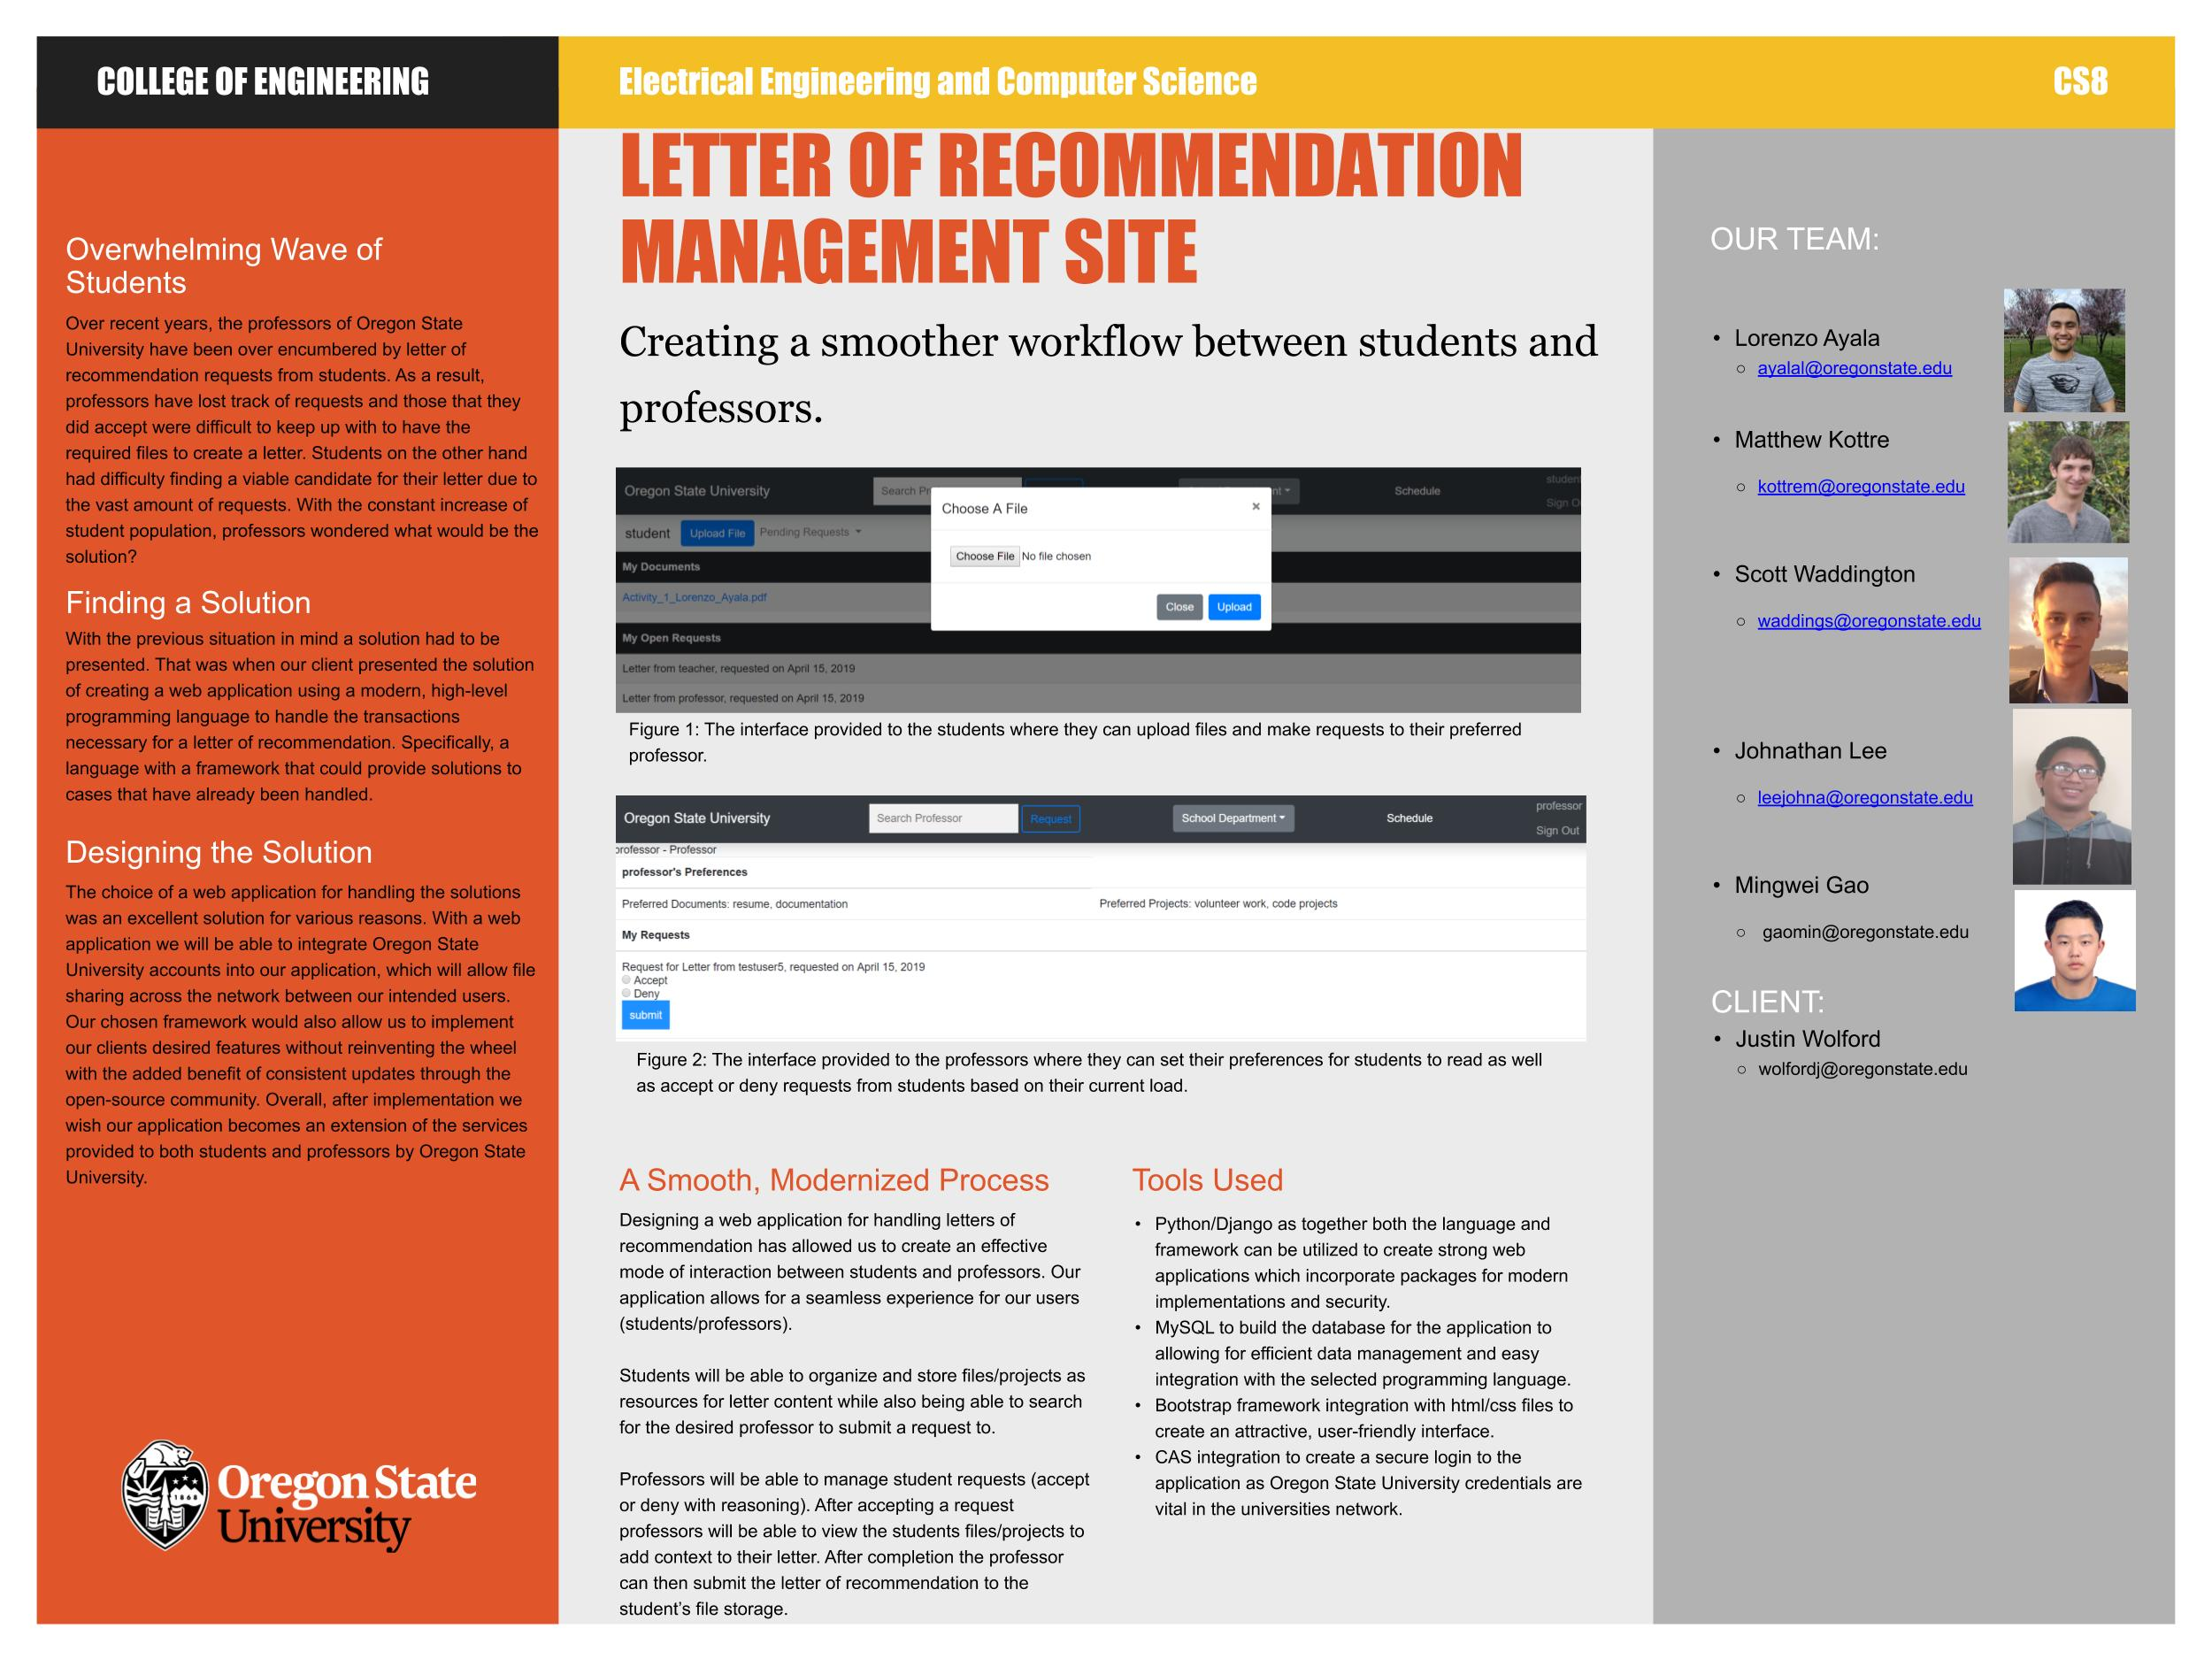
\includegraphics[angle=90,origin=c, width=15cm, height=20cm]{InputDocs/ExpoPoster.jpg}
		    \centering
	    \end{figure}
	\newpage
	
	\section{Project Documentation}

\subsection{Project Overview/Implementation}
\noindent The main operation of our project is to create a work flow between professors and students of Oregon State University when handling letters of recommendation. In order to connect the university to our application we integrated Oregon State's CAS login system so that professors and students can utilize there already existing accounts on our application. The application then provides two unique interfaces dependent on if the account is a student or professor. Students are provided a interface where they can upload files, search for a desirable letter candidate, and make requests through that previous search. Professors are able to set preferences for students to view so that the student is aware of what documentation to upload for that professor. Professors can also handle all letter requests from students via a accept/deny system which based on the decision will provide the necessary follow up. Should the recommendation be accepted the professor will have access to the students file which will allow the professor to begin working on the letter of recommendation. A schedule will also be created between both parties with a predetermined deadline for the letter and a description on the request. Should a request be denied the student will be sent an email stating that the specific professor has denied their request. After completing a letter a professor can then submit that letter to the specific student who can then use it for future use/reference.

\subsection{Software Installation/Operation}
\noindent Handling our project will be difficult for those who are outside the scope of our project since it relies on an AWS account between our group and the client. Permissions to this account can not be handed out either since the application uses sensitive information. However, they is a way to use the application from a local instance but with the caveat that not all features will be present and/or work correctly. In order to run the web application locally there are a few software requirements that are necessary to handle. First, the user will need to install a version of Python 3 and the python install pip3 to use the commands needed to run our application. In order to aid our users we created a install script that will handle the previous stated software installation as well as handle all package dependencies utilized with our application as python allows for the setup of a requirements text file which can be used as a dump for all package arguments for future installation on other systems. After completing the required installation the script will then run the application locally for the user via the command 'python3 manage.py runserver'. Should the user desire to stop the server they can 'ctrl-C' to stop then if they want to start the application back up simply run the 'python3 manage.py runserver' argument again to restart. In terms of a user guide we will have one listed on our Github repository for more in depth usage of our web application.    
	\newpage
	
	\section{Technical Resources}
    \subsection{Helpful Sites}
    \subsubsection{Official Django Documentation Site}
    \noindent The official documentation was a super useful site since it contained almost all the necessary information when dealing with the framework as well as adapting built in functions to an application. Django's site contains extensive information on each version that is released to the public and is based upon an open source community for package development which became extremely useful for our project.\\
    
    \subsubsection{Amazon Web Services Console and Documentation}
    \noindent Amazon Web Services was an essential site and service for our web application. Via Amazon's console and detailed guidelines we were able to utilize this service through Oregon State University for necessary development on our project such as implement CAS services to allow login with student and staff accounts. Amazon's detailed guides also provided us with quality information on creating an instance with their servers so that we could hit the ground running with our choice of operating systema long with dedicated memory and storage.\\
    
    \subsubsection{Stack Overflow Website}
    \noindent We would like to credit the website Stack Overflow since we consolidated a number of posts that dealt with web application development to handle numerous issues that others have faced in the past. Seeing previous suggestions, solutions, and advice provided us with numerous learning opportunities while solving issues that we faced during the development of our project. 
    
    \subsection{Helpful Personnel}
    \subsubsection{Justin Wolford}
    \noindent Our client Justin was a great resource to have for our project. He provided quick and effective communication with the team while also providing valuable feedback. Justin also helped point us in the right direction when questioning certain implementations. Justin was also essential in aiding us for contacting the OSU CAS team and providing resources to create an account with Amazon Web Services.\\
    
    \subsubsection{OSU CAS Team}
    \noindent The OSU CAS Team was a great team to work with as they provided fast communication in setting us up with a development server to utilize CAS into our web application. Integration was smooth and effective making for a very pleasurable experience.\\
    
    
    
	\newpage
	
	\section{Team Member Reflections}
\subsection{Lorenzo Ayala}\\
\subsubsection{What technical information did you learn?}
\noindent Over the duration of this project I learned just how extensive a web application can become even from the perspective of adding a micro-service to an existing organization. I also learned one of the most utilized frameworks.\\

\subsubsection{What non-technical information did you learn?}
\noindent In terms of non-technical aspects I learned what can be expected from projects in terms of documentation and preparing the necessary paperwork which can provide a strong analysis on your product while also being a guide on how the product operates. Also time management is key when handling large projects such as this.\\ 

\subsubsection{What have you learned about project work?}
\noindent I learned that delegation of tasks is essential in developing a product since it is always easier to conquer an issue broken up in smaller problems to solve rather than trying to solve them by yourself head on. In relation to delegating tasks, always match up tasks with team member strengths for efficiency and effectiveness of solutions.\\ 

\subsubsection{What have you learned about project management?}
\noindent Similar to the non-technical information, time management is key when it comes to large projects such as this one. Projects for senior capstone are ones that can't be done the weekend before it takes determination, efficiency, and work ethic to create a product to be proud of. Also, as I said before delegate tasks among your group to match strengths and avoid weaknesses to be an efficient group that is enjoying working on the project. I believe that these reasons are why we had a good time working on our project. Finally, I would like to add that do not be afraid to ask for help as there are so many helpful individuals at Oregon State University who could help you solve an issue in quick amount of time (rather than waste time trying to solve it yourself).\\

\subsubsection{What have you learned about working in teams?}
\noindent Having previously work at Cambia Health Solutions I was accustomed to working with teams on an industry level so I was able to sharpen the skills I learned from them. Following that statement, always go in with an open mind it is great seeing the various solutions and implementations your teammates come up with and can provide you with an alternative perspective you may have missed otherwise. Communication with each other is essential and can determine how development can go as well as other aspects of the project. Lastly, have fun with one another it makes the entire project enjoyable and memorable!\\

\subsubsection{If you could do it all over, what would you do differently?}
\noindent Probably have more courage to ask for help when I needed it while working on the project. I tend to shy away from help since it makes me feel as if I failed to implement some aspect of the project. Erasing this type of mindset was huge since asking for help from others provided quick solutions while giving me learning opportunities from individuals who have a wide array of knowledge in computer science. Also, if you can, start your project as early as possible. While we did not wait last minute to do our project we didn't start as soon as possible and that time could have been used to make something even more spectacular. Finally once again have fun this is a great learning experience and a way to introduce yourself to professionals within/outside Oregon State University.\\

\subsection{Johnathan Lee}\\

\subsubsection{What technical information did you learn?}
\noindent Some technical information I learned over the course of the year was learning how to code in Django environment and utilizing its database. I got to experience making a website from the bottom up and develop it from scratch. It was a nice experience learning how to make a website coding in Python because it is different from coding in C style languages.\\

\subsubsection{What non-technical information did you learn?}
\noindent Some of the non-technical information that I learned about included keeping track of documentation and recording daily progress on a huge project. It really puts in perspective what was done over the course of the year. \\ 

\subsubsection{What have you learned about project work?}
\noindent I have learned that big projects can have a lot of work involved and that teammates need to communicate clearly to properly cover the entire scope of the project. Overlapping or missing parts from the project could cause confusion within the team and hinder progress.\\ 

\subsubsection{What have you learned about project management?}
\noindent Some things that I learned about project management is that it’s a lot easier when there is a team leader coordinating the project. Things can quickly fall apart when there’s a lack of communication between team members.\\

\subsubsection{What have you learned about working in teams?}
\noindent I learned that communication can be important in working in teams and that assumptions can never be made about anything so everything needs to be clearly expressed before confirmation.\\

\subsubsection{If you could do it all over, what would you do differently?}
\noindent If I could do it all over again, there is not too much that I would like to change. However, some things I would like to try is offering my teammates some help more proactively as an attempt to offload some of the work being shared.\\

\subsection{Matthew Kottre}\\
\subsubsection{What technical information did you learn?}
\noindent I learned a lot about Django and the structure of Model/View frameworks. I also became much more proficient in database management from fixing a few problems that Django did not handle correctly.\\

\subsubsection{What non-technical information did you learn?}
\noindent I learned just how much writing and documentation is involved with projects. We spent far more time planning and writing documentation than we did coding. I've always been the kind of person who procrastinates on work, and that was not going to work well with a large project like this. As a result, my organization and time management skills significantly improved.\\ 

\subsubsection{What have you learned about project work?}
\noindent I learned how important planning and organization is. In order for each team member to effectively complete their part, they need to know how and what everyone else is doing as well.\\ 

\subsubsection{What have you learned about project management?}
\noindent I learned just how much writing and documentation is involved with projects. We spent far more time planning and writing documentation than we did coding. I also learned the importance of organization and time management.\\

\subsubsection{What have you learned about working in teams?}
\noindent I learned how important planning and organization is. In order for each team member to effectively complete their part, they need to know how and what everyone else is doing as well.\\

\subsubsection{If you could do it all over, what would you do differently?}
\noindent I would have liked to show more initiative throughout the project by volunteering to do certain tasks rather than waiting to be assigned left-overs. I have always been reactive, rather than proactive, so this project was a wake-up call telling me that I need to start planning ahead rather than waiting and hoping everything works out.\\

\subsection{Scott Waddington}\\

\subsubsection{What technical information did you learn?}
\noindent As a CS Systems Option, I don't get a lot of in-depth exposure to any one particular aspect of Computer Science. Being a member of this team and working on a web development project introduced me to a lot of aspects in web design that I wasn't familiar with, having only CS 290 under my belt as far as web programming experience is concerned. I also became somewhat familiar with Django, which I haven't used before. I don't claim to be an expert, but I can say with a degree of confidence that I could build a functional website in the future, with the experience that I gained from this project.\\

\subsubsection{What non-technical information did you learn?}
\noindent Documentation was huge throughout the capstone series. While we certainly could improve on some of our documentation, for the most part I think that we did a good job recording our progress and changes made to the project along the way. While we have all had to complete many assignments as an undergraduate, this one is unique because there was no clear guidelines for what needed to be done and how to implement it. Our client essentially gave us free reign on how we chose to design the application. This added a level of difficulty that we, as undergrads, rarely get to experience. Many assignments are strictly laid-out and the requirements are clearly communicated. This project gave us the chance to set out own schedule, come up with realistic expectations, and a plan to follow through, as well as the understanding that not everything is going to be implemented according to the first plan. The key is to adapt and to set realistic goals, and meet them.\\

\subsubsection{What have you learned about project work?}
\noindent As I said above, the most important thing we learned is that no plan survives the first point of contact. In essence, even the best plans for a project might change once implementation starts. There are things that occur that no one could foresee, and it's important to know how to adapt and overcome these challenges.\\

\subsubsection{What have you learned about project management?}
\noindent Communication is really important to a team, especially because we all have different schedules, unlike a job where everyone shows up at the same time and works. We all have other classes that we need to pass in order to graduate, and other obligations to tend to, so being able to communicate to one another was key to completing the project. At the beginning, we relied a lot on online communication and interaction, and as expo became nearer, we started meeting in-person more often in order to finish the project.\\

\subsubsection{What have you learned about working in teams?}
\noindent Again, I learned how much of an impact communication has on a team's success. It is important to have clear expectations of team members as well, and to ask for help when you need. Some people have more experience than others on certain aspects of the project, so consult those who know more than you. I didn't know anything about databases throughout the majority of the design and development of the project, so anytime I had to work with the database or create models in Django, I knew I had to ask one of my teammates for input.\\

\subsubsection{If you could do it all over, what would you do differently?}
\noindent Specific to this project, I think we would start working on CAS and AWS early. Both of these aspects took way longer to implement than we had expected, and it delayed some of the other features of our project until just before expo. I think we should have also worried less about the database, as we came to find out that Django had a lot of database management features build in, including the use of forms and models to represent objects in the database. I also think that if we had a stronger, more solid design in the beginning, it would have been easier to implement the project in the end.\\

\subsection{Mingwei Gao}\\
\subsubsection{What technical information did you learn?}
\noindent The most valuable technical information i learn from our project is how to design the database design and implementation in Django. Especially, I learn pretty much more when using what I learn from my advanced database building the data system. The six-stage of the design process of DBMS I learn from other class being translated into practice when I doing our project. (system, concept, logic, physics, implement, operation and maintenance)\\

\subsubsection{What non-technical information did you learn?}
\noindent The non-technical information that I learned should be the standard Latex writing and how to make the complete, well-formed documents. Since I am not a good writer, usually I won't encourage me to participate in any key writing part when I am in the large project. The weekly process record in our class helps me resolve this problem. Becasue I know what I did every week and what's going to do next time, I can manage my time and learning clearly. In other words, I know what I should write even more thinking after I review my weekly process. So, my learning management significantly improved. \\ 

\subsubsection{What have you learned about project work?}
\noindent Except for the deeper understanding of the technical problems arising from such a large-scale project, I learned how to work efficiently in the team including my clients and teammates. Also,  the project schedule management is the key role in our project. Project schedule management is the foundation and the key management stage to ensure the successful implementation of a project. \\ 

\subsubsection{What have you learned about project management?}
\noindent Communicate with your team, client, as to how we can improve our project management practices. Recording the week process is an important aspect of project management performed throughout the project. \\

\subsubsection{What have you learned about working in teams?}
\noindent I have learned the way how to work effectively in collaborative project teams. Every member needs providing guidance, support or assistance with each other as appropriate. All member should have high responsibility and efficiency to schedule, organize and coordinate projects with team spirit. \\

\subsubsection{If you could do it all over, what would you do differently?}
\noindent If I could do it all over again, I would complete the task a little earlier once I have received the team's requirement.  Even now I have the deep procrastination in my daily life, I have started making my daily work more structured by working with people who have a good life habit. Obviously, my teammates all have good habits and positive attitudes, their behavior was affecting my future work performance. \\
	\newpage
	
	\section{Appendix 1}
\subsection{File Upload}
\noindent For handling file uploads we were able to use built in functionality that Django presented to us as a solution for handling file transfer to a web application. Django's function connects to the users operating system which then allows the user to choose which file they desire to upload. Below is the code block used to filter then allow the user to fill out the necessary form to upload a file which was made simple thanks to Django's built in functionality.\\ 
    \begin{lstlisting}
        current_user = request.user
    group = Group.objects.filter(user = request.user)
    if group.filter(name='Professors').exists():
        redir = "/professor_profiles/" + str(request.user.id)
        return redirect(redir)
    if request.method == 'POST':
        form = DocumentForm(request.POST, request.FILES)
        if form.is_valid():
            obj = form.save(commit=False)
            obj.user = request.user
            obj.save()
            return redirect('index')
    \end{lstlisting} \\
    
\subsection{CAS Implementation}
\noindent Integrating Oregon State University accounts into our application was very simple thanks to the opens source community that developed a CAS python package for online applications. Simple as it was we had some issues with integration as some of the development packages we were using prevented the CAS package from accessing the URL to the schools CAS developer server. After using some sources from stack overflow we realized there were some unneeded packages in our instance that we had to lean out as well as update other package versions. After cleaning up our dependencies we were then able to run CAS on our application by simplying using the few lines below in our settings.py file. 
        \begin{lstlisting}
        CAS_SERVER_URL = 'https://login.oregonstate.edu/cas-dev/'

        #CAS_PROXY_CALLBACK = 'http://18.223.30.206/accounts/callback'

        CAS_APPLY_ATTRIBUTES_TO_USER = True
        \end{lstlisting}
    

	
	
	
	

\end{document}